\documentclass{beamer}

\usepackage{amsmath}
\usepackage{amssymb}
\usepackage{tikz}
\usepackage{pgfplots}

\title{Least-Square Problem}
\subtitle{The ``Whole"  Point of Chapter 6}
\author{Ahmed Mohammed}
\institute{Georgia Institute of Technology}
\date{PLUS Session, Summer 2023}

\usetheme{Copenhagen}
\usefonttheme{serif}
\usecolortheme{seagull}

\renewcommand{\vec}[1]{\mathbf{#1}}
\DeclareMathOperator{\proj}{proj}
\DeclareMathOperator{\colspace}{Col}


% from https://tex.stackexchange.com/a/75550/227665
\makeatletter
\let\save@measuring@true\measuring@true
\def\measuring@true{%
  \save@measuring@true
  \def\beamer@sortzero##1{\beamer@ifnextcharospec{\beamer@sortzeroread{##1}}{}}%
  \def\beamer@sortzeroread##1<##2>{}%
  \def\beamer@finalnospec{}%
}
\makeatother

\AtBeginSection[]
{
    \begin{frame}
        \frametitle{Table of Contents}
        \tableofcontents[currentsection]
    \end{frame}
} % https://statisticaloddsandends.wordpress.com/2019/02/18/beamer-inserting-section-slides-before-each-section/

\begin{document}
	\begin{frame}
		\maketitle
	\end{frame}

	\section{Open Activity: Review}
	\begin{frame}
		\frametitle{Motivation}
		In many circumstances, we may not be able to solve the matrix equation \(A\vec{x} = \vec{b}\). \pause

		We then opt to solving the equation \(A\vec{\hat{x}} = \vec{\proj}_{\colspace A} \vec{b} = \vec{\hat{b}}\), which we know is \emph{always} consistent. \pause

		\begin{definition}
			Each solution \(\vec{\hat{x}}\) of the equation \(A\vec{\hat{x}} = \vec{\hat{b}}\) is called a \emph{least-square solution.} \pause
		\end{definition}
			
		\textit{Remark:} There might be more than one least-square solution.
	\end{frame}

	\begin{frame}
		\frametitle{Motivation \textit{Cont.}}
		We basically find the best approximation for our vector \(\vec{b}\) in \(A\vec{x} = \vec{b}\) and solve for \(A\vec{\hat{x}} = \text{approx. of } \vec{b}\). We use the Best Approximation Theorem to find the best approximation of \(\vec{b}\).
		\begin{theorem}
			If \(W \subset \mathbb{R}^{n}\), and \(\vec{y} \in \mathbb{R}^n\), then 
			\[\|\operatorname{proj}_W\vec{y} - \vec{y} \| < \|\vec{w} - \vec{y}\|\]
			for any \(\vec{w} \in W\) with \(\vec{w} \ne \operatorname{proj}_W\vec{y}.\)
		\end{theorem}
	\end{frame}

	\begin{frame}
		\frametitle{Motivation \textit{Cont.}}
		Calculating the projection of a vector onto a subspace is really simple! \pause 
		\begin{align*}
			\proj_{\colspace A} \vec{b} &= \frac{\vec{a}_1 \cdot \vec{b}}{\vec{a}_1 \cdot \vec{a}_1}\vec{a}_1 + \frac{\vec{a}_2 \cdot \vec{b}}{\vec{a}_2 \cdot \vec{a}_2}\vec{a}_2 + \cdots + \frac{\vec{a}_p \cdot \vec{b}}{\vec{a}_p \cdot \vec{a}_p}\vec{a}_p \\[0.5em] \pause
								 &= \underbrace{\begin{bmatrix}\vec{a}_1 & \vec{a}_2 & \dots & \vec{a}_p\end{bmatrix}}_{A}\underbrace{\begin{bmatrix}\frac{\vec{a}_1 \cdot \vec{b}}{\vec{a}_1 \cdot \vec{a}_1} \\[0.5em] \frac{\vec{a}_2 \cdot \vec{b}}{\vec{a}_2 \cdot \vec{a}_2} \\[0.5em] \vdots \\[0.5em] \frac{\vec{a}_p \cdot \vec{b}}{\vec{a}_p \cdot \vec{a}_p}\end{bmatrix}}_{\vec{\hat{x}}} = \vec{\hat{b}} \pause
		\end{align*}

		We've found the vector \(\vec{\hat{x}}\) such that \(A\vec{\hat{x}} = \vec{\hat{b}}\). So, are we done? 
	\end{frame}

	\begin{frame}
		\frametitle{Motivation \textit{Cont.}}
		No! 
		\begin{enumerate}
			\item<2-> Works for \emph{orthogonal basis} only, not \emph{any} basis.
			\item<3-> We have no guarantee that the columns of \(A\) are linearly independent, let alone orthogonal.
		\end{enumerate}

		\onslide<4->{We have two options:}
		\begin{enumerate}
			\item<4-> Try to apply Gram-Schmidt to the columns of \(A\) and from there use the projection formula. 
					\color{red}(Read the erratum.)\color{black}
			\item<5-> Find a workaround.
		\end{enumerate}
	\end{frame}

	\begin{frame}
		\frametitle{The Work Around: The Normal Equations}
		\begin{itemize}
			\item<1-> Using Gram-Schmidt is tedious and long. \color{red}(Read the erratum.)\color{black}
			\item<2-> Using the Normal Equations is easier and simpler. 
		\end{itemize}

		\onslide<3->{
			\[A^TA\vec{x} = A^T\vec{b}.\]
		}

		\onslide<4->{
			Turns out that each vector \(\vec{x}\) satisfying the above equation also satisfies the equation \(A\vec{x} = \proj_{\colspace A} \vec{b}\).
		}

		\onslide<5->{
			Therefore, a solution to the norm equations \emph{also} count as a least-square solution.
		}
	\end{frame}
	
	\section{Application}
	\begin{frame}
		\frametitle{Use}
		Least-square problems come up in simple \emph{linear regression} problems. \pause

		\begin{enumerate}
			\item<2-> We have data points \((x_1, y_1), (x_2, y_2), \dots, (x_n, y_n)\) that we wish to connect with curve.
			\item<3-> We chose a linear model. For example, \(y_i = \beta_0 + \beta_1 x_i\) or \(y_i = \beta_0 + \beta_1 x_i^2\).
			\item<4-> We try to find what values for \(\beta_i\) will yield the graph with the least amount of ``error".
		\end{enumerate}
	\end{frame}
	
	\begin{frame}
		\frametitle{Example}
		Find the values for \(\beta_0, \beta_1\) that'll best fit the curve \[y = \beta_0 + \beta_1 x\] to the data points \((1, 2), (2, 3), (3, 3), (5, 5)\). \pause

		\begin{figure}[!h]
			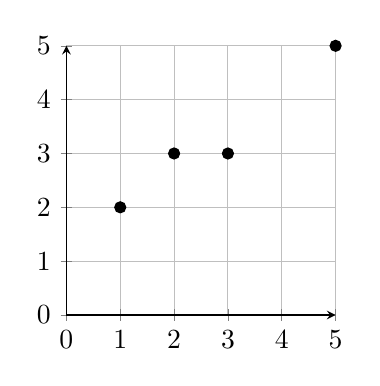
\begin{tikzpicture}
				\begin{axis}[axis lines = left, grid=major, height=5cm, width = 5cm, xmin=0, xmax=5, ymin=0, ymax=5, xtick distance = 1, ytick distance = 1]
					\plot[mark=*, only marks, black] coordinates {(1, 2) (2, 3) (3, 3) (5, 5)};
				\end{axis}
			\end{tikzpicture}
		\end{figure}
	\end{frame}

	\begin{frame}
		\frametitle{Example \textit{Cont.}}
		Find the values for \(\beta_0, \beta_1\) that'll best fit the curve \[y = \beta_0 + \beta_1 x\] to the data points \((1, 2), (2, 3), (3, 3), (5, 5)\).
		\begin{figure}[!h]
			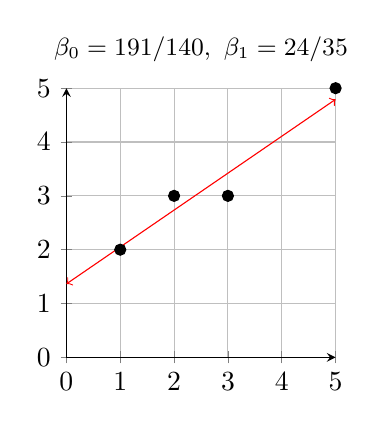
\begin{tikzpicture}
				\begin{axis}[axis lines = left, grid=major, height=5cm, width = 5cm, xmin=0, xmax=5, ymin=0, ymax=5, xtick distance = 1, ytick distance = 1, title={\small \(\beta_0 = 191/140, \ \beta_1 = 24/35\)}]
					\plot[mark=*, only marks, black] coordinates {(1, 2) (2, 3) (3, 3) (5, 5)};
					\addplot[<->, red, domain=0:5] {191/140 + 24/35 * x};
				\end{axis}
			\end{tikzpicture}
		\end{figure}
	\end{frame}

	\begin{frame}
		\frametitle{Model Choice}
		Note that a different model could've been chosen for the previous problem, and as long as the model is linear in the parameters, nothing of the steps would change.
	\end{frame}

	\section{Main Activity}
	\begin{frame}
		\frametitle{Exam Review!}
		Look at the worksheet!
	\end{frame}

	\begin{frame}
		\frametitle{Erratum}
		During the session, I implied that you can use the Gram-Schmidt process to solve for the projection of the vector \(\vec{b}.\) While this isn't 
		necessarily wrong, we won't be able to find solutions to \(A\vec{\hat{x}} = \vec{\hat{b}}\) using this method. 
		
		Say the columns of \(A\) are not orthogonal, and \(Q\) is the result of applying Gram-Schmidt to them. We will be able to solve 
		\(Q\vec{\hat{x}} = \vec{\hat{b}}\) quite easily using the projection formula. \emph{However}, we wouldn't be able to solve 
		\(A\vec{\hat{x}} = \vec{\hat{b}}\). That is, a solution to \(Q\vec{\hat{x}} = \vec{\hat{b}}\) won't yield a solution to 
		\(A\vec{\hat{x}} = \vec{\hat{b}}\) (and vice versa). 

		In conclusion, if you want to solve \(A\vec{\hat{x}} = \vec{\hat{b}}\), you'll \emph{need} to solve \(A^TA\vec{\hat{x}} = A^T\vec{b}\).
	\end{frame}
\end{document}
